\documentclass{article}

\usepackage{ctex}
\usepackage{amsmath,amssymb}
\usepackage{fancyhdr}
\usepackage[bookmarks=true,colorlinks,linkcolor=black]{hyperref}
\usepackage{fontspec}
\usepackage{tabularx,multirow,makecell}
\usepackage{listings,xcolor}
\lstset{
	language=C++,
	basicstyle=\ttfamily,
	numbers=left,numberstyle=\ttfamily,
	breaklines=true,
	tabsize=2
}
\usepackage{tikz}

\title{qhfz 算法思维训练\ 题解}
\author{registerGen}
\date{}

\pagestyle{fancy}
\fancyhead[L]{\leftmark}
\fancyhead[R]{qhfz 算法思维训练\ 题解}
\fancyfoot[C]{\thepage}

\setmonofont{Consolas}

\begin{document}
	\maketitle

	\tableofcontents
	
	\newpage

	\section{字串变换}

	\subsection{题目描述}

	给定一个由字符 \texttt{0},\texttt{1},\texttt{2} 组成的字符串 $s$。如果 \texttt{0} 和 \texttt{1} 相邻或 \texttt{1} 和 \texttt{2} 相邻,则我们可以交换它们的位置,如 \texttt{01} $\to$ \texttt{10},\texttt{10} $\to$ \texttt{01},\texttt{12} $\to$ \texttt{21} 等。

	对于 $s$,只可以进行上述操作,且可以操作任意的次数,请问可以得到的字典序最小的字符串是什么?

	\subsection{输入格式}

	一行,一个字符串 $s$。

	\subsection{输出格式}

	一行,表示答案。

	\subsection{输入输出样例}

	\begin{tabularx}{\textwidth}{|X|X|}
		\hline
		\textbf{输入 \texttt{\#}1} & \textbf{输出 \texttt{\#}1} \\
		\hline
		\texttt{100210} & \texttt{001120} \\ 
		\hline
		\textbf{输入 \texttt{\#}2} & \textbf{输出 \texttt{\#}2} \\
		\hline
		\texttt{11222121} & \texttt{11112222} \\ 
		\hline
	\end{tabularx}

	\subsection{说明/提示}

	\subsubsection{数据范围}

	对于 30\% 的数据,$|s|\le 10$。

	对于 50\% 的数据,$|s|\le 100$。

	对于 70\% 的数据,$|s|\le 10^{3}$。

	对于 100\% 的数据,$1\le |s|\le 10^{5}$,$\Sigma\subseteq\{\texttt{0},\texttt{1},\texttt{2}\}$。

	$|s|$ 表示字符串 $s$ 的长度,$\Sigma$ 表示字符集。

	\newpage

	\subsection{题解}

	由于 \texttt{0},\texttt{2} 的相对位置不会改变,所以只需将所有的 \texttt{1} 移到 $s$ 的第一个 \texttt{2} 前面即可。

	时间复杂度 $\mathcal O(n)$。

	\subsection{代码}

	\begin{lstlisting}
#include<cstdio>
#include<algorithm>
#include<cstring>

const int N=1e5;

int n;
char s[N+10];

int main(){
	scanf("%s",s+1);
	n=int(strlen(s+1));
	int pos=n+1,cnt=0; // pos 表示第一个 2 的位置,cnt 表示 1 的个数
	for(int i=1;i<=n;i++)
		if(s[i]=='1')cnt++;
	for(int i=1;i<=n;i++)
		if(s[i]=='2'){pos=i;break;}
	for(int i=1;i<pos;i++)
		if(s[i]!='1')putchar(s[i]);
	for(int i=1;i<=cnt;i++)
		putchar('1');
	for(int i=pos;i<=n;i++)
		if(s[i]!='1')putchar(s[i]);
	puts("");
	return 0;
}
	\end{lstlisting}

	\newpage

	\section{最大子方阵}

	\subsection{题目描述}

	给定 $n\times m$ 的矩形的点方阵,每个元素只可能为 1 或 0,例如:

	\begin{center}
		0111

		1000

		0110
	\end{center}
	
	1 表示这个位置上站着一位同学,0 表示这个位置上没有人。现在你有指挥的权利,具体为可以交换任意的两行,并且这个权利可以使用无数次,那么请问,你可以折腾指挥出一个最大的,全部由同学构成的子方阵吗?
	
	“子方阵”是指这样的点集:对于其中的任意一个点 $(x,y)$,$1\le a\le x\le b\le n,1\le c\le y\le d\le m$。子方阵的大小是指其中 1 的个数。

	例如,对于上述方阵,当 $a=1,b=2,c=2,d=3$ 时,子方阵为:

	\begin{center}
		11

		00
	\end{center}


	\subsection{输入格式}

	第一行包含 2 个整数 $n$ 和 $m$。

	接下来 $n$ 行,每行 $m$ 个字符,表示这一行中同学的分布情况。

	\subsection{输出格式}

	一行一个整数,表示答案。

	\subsection{输入输出样例}

	\begin{tabularx}{\textwidth}{|X|X|}
		\hline
		\textbf{输入 \texttt{\#}1} & \textbf{输出 \texttt{\#}1} \\
		\hline
		\texttt{3 4} & \texttt{4}\\
		\texttt{0111} & \\
		\texttt{1000} & \\
		\texttt{0110} & \\
		\hline
	\end{tabularx}

	\subsection{说明/提示}

	\subsubsection{样例 1 解释}

	我们可以交换原始方阵的 2,3 行,获得:

	\begin{center}
		0111

		0110

		1000
	\end{center}

	则当 $a=1,b=2,c=2,d=3$ 时,对应的子方阵即为最大子方阵。

	\subsubsection{数据范围}

	对于 50\% 的数据,$n,m\le 100$。

	对于 100\% 的数据,$1\le n,m\le 5\times 10^{3}$。

	\subsection{题解}

	首先,这个数据范围是允许我们枚举子方阵的一条边的,考虑枚举子方阵的左边。

	那么,我们可以“利用”的 1 的范围如下图:

	\begin{center}
		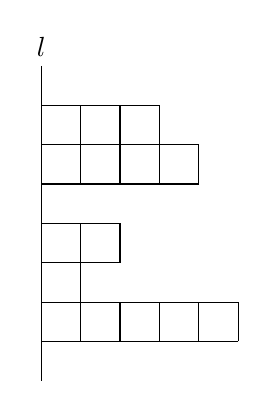
\begin{tikzpicture}[scale=0.5]
			\node[above] at (0,4) {$l$};
			\draw (0,4) -- (0,-4);
			\draw (0,2) grid (3,3);
			\draw (0,1) grid (4,2);
			\draw (0,-1) grid (2,0);
			\draw (0,-2) grid (1,-1);
			\draw (0,-3) grid (5,-2);
		\end{tikzpicture}
	\end{center}

	可以发现,第 $i$ 行可“利用”的 1 的个数为 $(i,l)$ 往右的连续的 1 的个数(包括它自己),记为 $b_{i,l}$。
	
	然后我们发现貌似还是不太好算,所以再枚举子方阵的右边。

	此时,由于行是可以随便换的,所以我们可以“利用”的 1 的范围如下图的红色部分:

	\begin{center}
		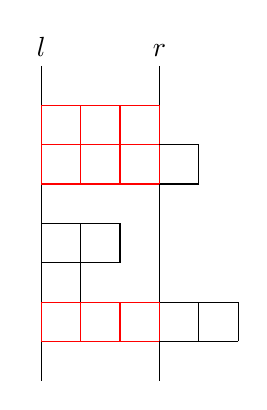
\begin{tikzpicture}[scale=0.5]
			\node[above] at (0,4) {$l$};
			\node[above] at (3,4) {$r$};
			\draw (0,4) -- (0,-4);
			\draw (3,4) -- (3,-4);
			\draw[color=red] (0,2) grid (3,3);
			\draw (3,1) grid (4,2);
			\draw[color=red] (0,1) grid (3,2);
			\draw (0,-1) grid (2,0);
			\draw (0,-2) grid (1,-1);
			\draw (3,-3) grid (5,-2);
			\draw[color=red] (0,-3) grid (3,-2);
		\end{tikzpicture}
	\end{center}

	为了方便计算,我们按 1 的个数从大到小排个序再枚举。

	现在的问题就是,如何高效计算 $b_{i,j}$?

	\begin{lstlisting}
for(int i=1;i<=n;i++){ // 对于每一行
	int cnt=0; // counter
	for(int j=m;j;j--){ // 倒着枚举
		if(a[i][j]==0)cnt=0; // 如果这个格子为 0 ,则 b[i][j] 就为 0
		else cnt++; // 如果这个格子为 1 ,则 b[i][j] = b[i][j+1] + 1 (即 cnt + 1 )
		b[i][j]=cnt;
	}
}
	\end{lstlisting}

	时间复杂度 $\mathcal O(nm\log n)$。但待排序的元素均在 $[0,m]$ 内,所以排序可以使用桶排,时间复杂度 $\mathcal O(nm)$。

	\subsection{代码}

	\begin{lstlisting}
#include<cstdio>
#include<algorithm>

const int N=5000;

int n,m;
bool a[N+10][N+10];
int b[N+10][N+10];
int tmp[N+10];
int buc[N+10];

int main(){
	scanf("%d%d",&n,&m);
	for(int i=1;i<=n;i++)
		for(int j=1;j<=m;j++)
			scanf("%1d",a[i]+j);
	// 预处理 b[i][j]
	for(int i=1;i<=n;i++){
		int cnt=0;
		for(int j=m;j;j--){
			if(a[i][j]==0)cnt=0;
			else cnt++;
			b[i][j]=cnt;
		}
	}
	int ans=0;
	for(int j=1;j<=m;j++){
		// tmp[i] 为 b[i][j] 排好序后的数组
		for(int i=1;i<=n;i++)tmp[i]=b[i][j];
		// 桶排
		for(int i=0;i<=m;i++)buc[i]=0;
		for(int i=n;i>=1;i--)buc[tmp[i]]++;
		int tot=0;
		for(int i=m;i>=0;i--)
			for(int k=1;k<=buc[i];k++)
				tmp[++tot]=i;
		int res=0;
		for(int i=1;i<=n;i++)
			res=std::max(res,i*tmp[i]); // 计算全部由同学构成的子方阵大小。如果不理解这句话可以画画图。
		ans=std::max(ans,res);
	}
	printf("%d\n",ans);
}
	\end{lstlisting}

	\newpage

	\section{摘苹果}

	\subsection{题目描述}

	果园中有 $n$ 棵苹果树,它们排成了一排,每棵树上有 $c_{i}$ 个苹果。现在,小玉站在第一棵树下,有 $W$ 点能量,同时能量上限也为 $W$。

	对于第 $i$ 棵树,小玉可以摘 $[0,c_{i}]$ 间的任意数量的苹果。\textbf{每摘一个} 苹果,小玉的能量将会被消耗 $cost_{i}$,但是能量上限将会增加 $B$。

	小玉只能按着顺序从第 1 棵树移动到第 2 棵树,从第 2 棵树到第 3 棵树……每次他到达下一棵树时,他都会恢复 $X$ 点能量(当然,不能超过当时的上限)。这样一直进行下去,请问最后小玉最多可以摘到多少苹果?注意,小玉不可以出现负能量的状态。

	\subsection{输入格式}

	第一行 4 个整数 $n,W,B,X$。

	第二行 $n$ 个整数 $c_{i}$。

	第三行 $n$ 个整数 $cost_{i}$。

	\subsection{输出格式}

	一行一个整数表示答案。

	\subsection{输入输出样例}

	\begin{tabularx}{\textwidth}{|X|X|}
		\hline
		\textbf{输入 \texttt{\#}1} & \textbf{输出 \texttt{\#}1} \\
		\hline
		\texttt{2 10 7 11} & \texttt{11} \\
		\texttt{2 10} & \\
		\texttt{6 1} & \\
		\hline
		\textbf{输入 \texttt{\#}2} & \textbf{输出 \texttt{\#}2} \\
		\hline
		\texttt{5 1 4 6} & \texttt{10} \\ 
		\texttt{3 4 6 5 1} & \\
		\texttt{3 0 10 2 9} & \\
		\hline
	\end{tabularx}

	\subsection{说明/提示}

	\subsubsection{数据范围}

	对于 40\% 的数据,$1\le n\le 100$,$\displaystyle 1\le \sum_{i=1}^{n} c_{i} \le 100$。
	
	对于 100\% 的数据,$1\le n\le 10^{3}$,$\displaystyle 1\le \sum_{i=1}^n c_{i} \le 10^{4}$,$0\le c_{i}\le 10^{4}$,$0\le W,B,X,cost_{i}\le 10^{9}$。

	\subsection{题解}

	首先,容易想到如下的状态设计:设 $f_{i,j}$ 表示只摘前 $i$ 棵树上的苹果,且当前能量为 $j$ 时能摘到的最多的苹果。

	很快你会发现这很不现实—— $W\le 10^9$,我们不能开下这么大的数组!

	考虑从 $\displaystyle\sum_{i=1}^n c_i\le 10^4$ 入手,改变状态如下:

	设 $f_{i,j}$ 表示前 $i$ 棵树,摘了 $j$ 个苹果的——等等,摘了 $j$ 个苹果的什么呀?

	考察题目的变量,你会发先有三个:摘了的 苹果树 的个数,摘到的 苹果 的个数,能量。

	\begin{quote}
		dp 第 $\times$ 定理:一般的,设计状态时要把题目中所有变量包含进状态里。
	\end{quote}

	那么,我们可以得到最终的状态定义:\textbf{设 $f_{i,j}$ 表示前 $i$ 棵树,摘了 $j$ 个苹果的最大能量}(当然是能量越多越好了)。

	那么,最终的答案就是使得 $f_{n,i}\ge 0$ 的最大的 $i$。

	有了状态定义,转移方程和初始化就很简单了:

	\[
		f_{i,j}=\max_{k\in[0,c_i]}\{\min\{f_{i-1,j-k}-k\cdot cost_i+X,W+jB\}\}\quad\text{if }f_{i-1,j-k}-k\cdot cost_i \ge 0
	\]

	初始化:

	\[
		f_{i,j}=\begin{cases}W&i=0\land j=0\\-\infty&\text{otherwise}\end{cases}
	\]

	开一个 $10^3\times 10^4$ 的 \texttt{long long} 数组可能会爆空间(我懒得算),可以滚动数组优化空间。

	Upd:刚算了一下,不会炸。

	\[
		\text{所需空间 }=\frac{10^{3}\times 10^{4}\times 8}{1024\times 1024}\approx 80\text{ MB}
	\]

	时间复杂度 $\displaystyle\mathcal O\left(\left(\sum_{i=1}^n c_{i}\right)^2\right)$。

	\subsection{代码}

	\begin{lstlisting}
#include<cstdio>
#include<algorithm>
#include<cstring>

typedef long long ll;

const int N=1e3;
const int M=1e4;
const ll inf=0x3f3f3f3f3f3f3f3fLL;

int n,W,B,X,c[N+10],cost[N+10],sumc;
ll f[2][M+10]; // 不滚动: f[N+10][M+10];

int main(){
	scanf("%d%d%d%d",&n,&W,&B,&X);
	for(int i=1;i<=n;i++)
		scanf("%d",c+i),sumc+=c[i];
	for(int i=1;i<=n;i++)
		scanf("%d",cost+i);
	memset(f,~0x3f,sizeof(f));
	f[0][0]=W;
	for(int i=1;i<=n;i++)
		for(int j=0;j<=sumc;j++)
			for(int k=0;k<=std::min(c[i],j);k++){
				ll tmp=f[(i&1)^1][j-k]-1LL*k*cost[i]; // 不滚动: f[i-1][j-k]-1LL*k*cost[i]
				if(tmp<0)continue;
				tmp+=X;
				if(tmp>W+1LL*j*B)tmp=W+1LL*j*B;
				f[i&1][j]=std::max(f[i&1][j],tmp); // 不滚动: f[i][j]=std::max(f[i][j],tmp)
			}
	for(int i=sumc;~i;i--)
		if(f[n&1][i]>=0){
			printf("%d\n",i);
			return 0;
		}
	return 0;
}
	\end{lstlisting}

	\newpage
	
	\section{宝石圆盘}

	\subsection{题目描述}

	给定一个 $n$ 个数的数列 $a$。定义一次操作为,删掉一个 $a$ 的 \textbf{连续} 回文子序列 $[a_l,a_{l+1},\cdots,a_r]$,然后令 $a\gets [a_1,a_2,\cdots,a_{l-1},a_{r+1},a_{r+2},\cdots]$。

	现在你要把这个序列删成空序列,求最小的操作次数。

	一个序列 $b=[b_1,b_2,\cdots,b_m]$ 是回文的,当且仅当 $b_1=b_m,b_2=b_{m-1},\cdots,b_m=b_1$。

	\subsection{输入格式}

	第一行一个整数 $n$。

	第二行 $n$ 个整数,第 $i$ 个整数表示 $a_i$。

	\subsection{输出格式}

	一行一个整数表示答案。

	\subsection{输入输出样例}

	\begin{tabularx}{\textwidth}{|X|X|}
		\hline
		\textbf{输入 \texttt{\#}1} & \textbf{输出 \texttt{\#}1} \\
		\hline
		\texttt{8} & \texttt{2} \\
		\texttt{1 2 1 3 4 1 2 1} & \\
		\hline
	\end{tabularx}

	\subsection{说明/提示}

	\subsubsection{样例 1 解释}

	首先删掉 $a_4(=3)$,此时 $a=[1,2,1,4,1,2,1]$,然后将现在的 $a$ 全部删掉即可。

	\subsubsection{数据范围}

	对于测试点 $1\sim 3$,$n\le 10$。

	对于测试点 $4\sim 5$,$n\le 100$。

	对于测试点 $6\sim 10$,$n\le 500$。

	对于 100\% 的数据,$1\le n\le 500$,$1\le a_i\le n$。
\end{document}
